% Pdf only
\documentclass[aspectratio=169]{beamer}
% For presentation
%\documentclass[aspectratio=169, notes]{beamer}
\usepackage{lmodern}
\usepackage{pgfpages}
%\setbeameroption{show notes on second screen}
%\usepackage[utf8]{inputenc} 
\usepackage[english]{babel}

%
% Choose how your presentation looks.
%
% For more themes, color themes and font themes, see:
% http://deic.uab.es/~iblanes/beamer_gallery/index_by_theme.html
%
\mode<presentation>
{
  \usetheme[]{metropolis}           % Use metropolis theme
} 

\begin{document}
\obeylines

\title[ORB SLAM Point Cloud generation on Apalis iMX8]{ORB SLAM Point Cloud generation on Apalis iMX8}
\author{Stefan Eichenberger, CPVR Lab}
\date{25.01.2019}


\begin{frame}
  \titlepage\thispagestyle{empty}
\end{frame}

\note[itemize]{
\item Herzlich wilkommen zur Präsentation über ORB Slam Point Cloud generation on Apalis iMX8
\item Wer von euch hat zuhause einen Staubsaugerroboter?
\item Wer findet der ist super intelligent?
}

\begin{frame}{Why SLAM}
  \begin{center}
    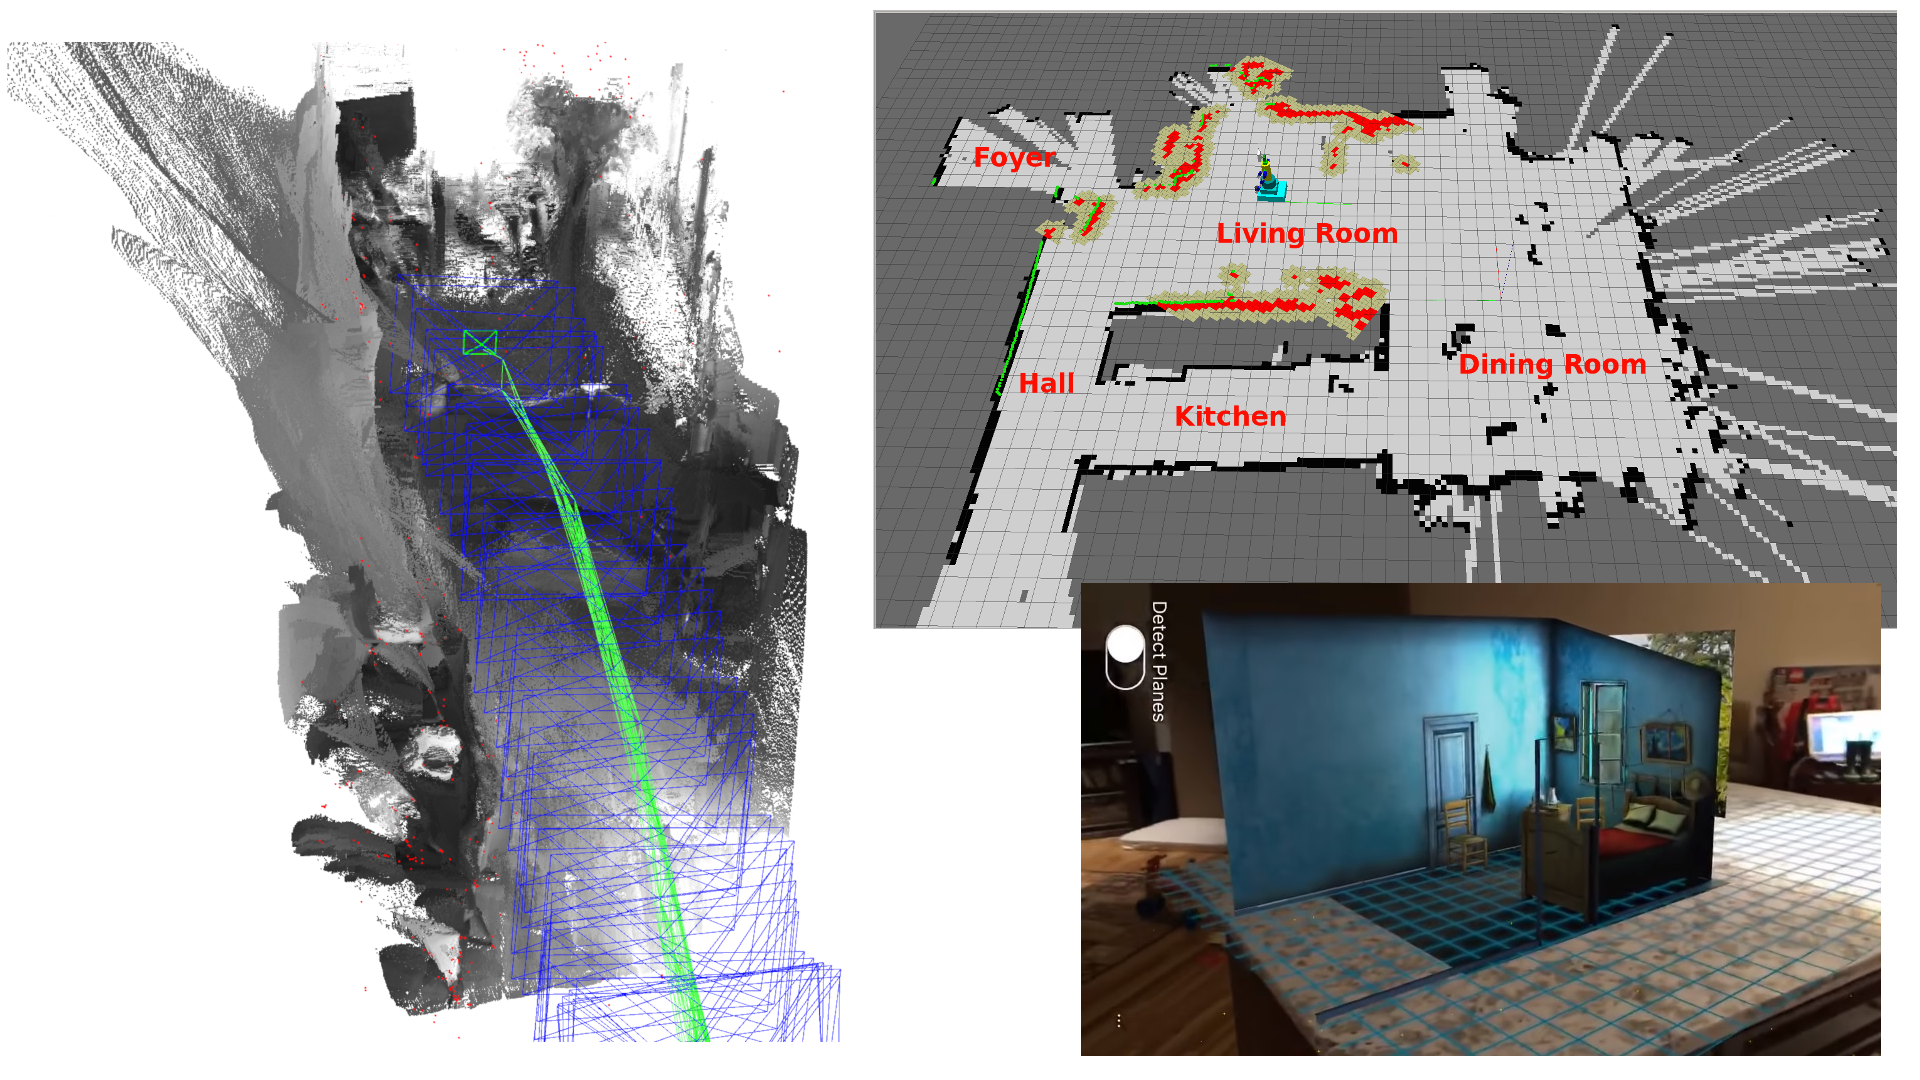
\includegraphics[height=0.9\textheight]{./img/slam_usecases.png}
  \end{center}
\end{frame}

\note{
}

\begin{frame}{Toradex Apalis iMX8}
  \begin{center}
    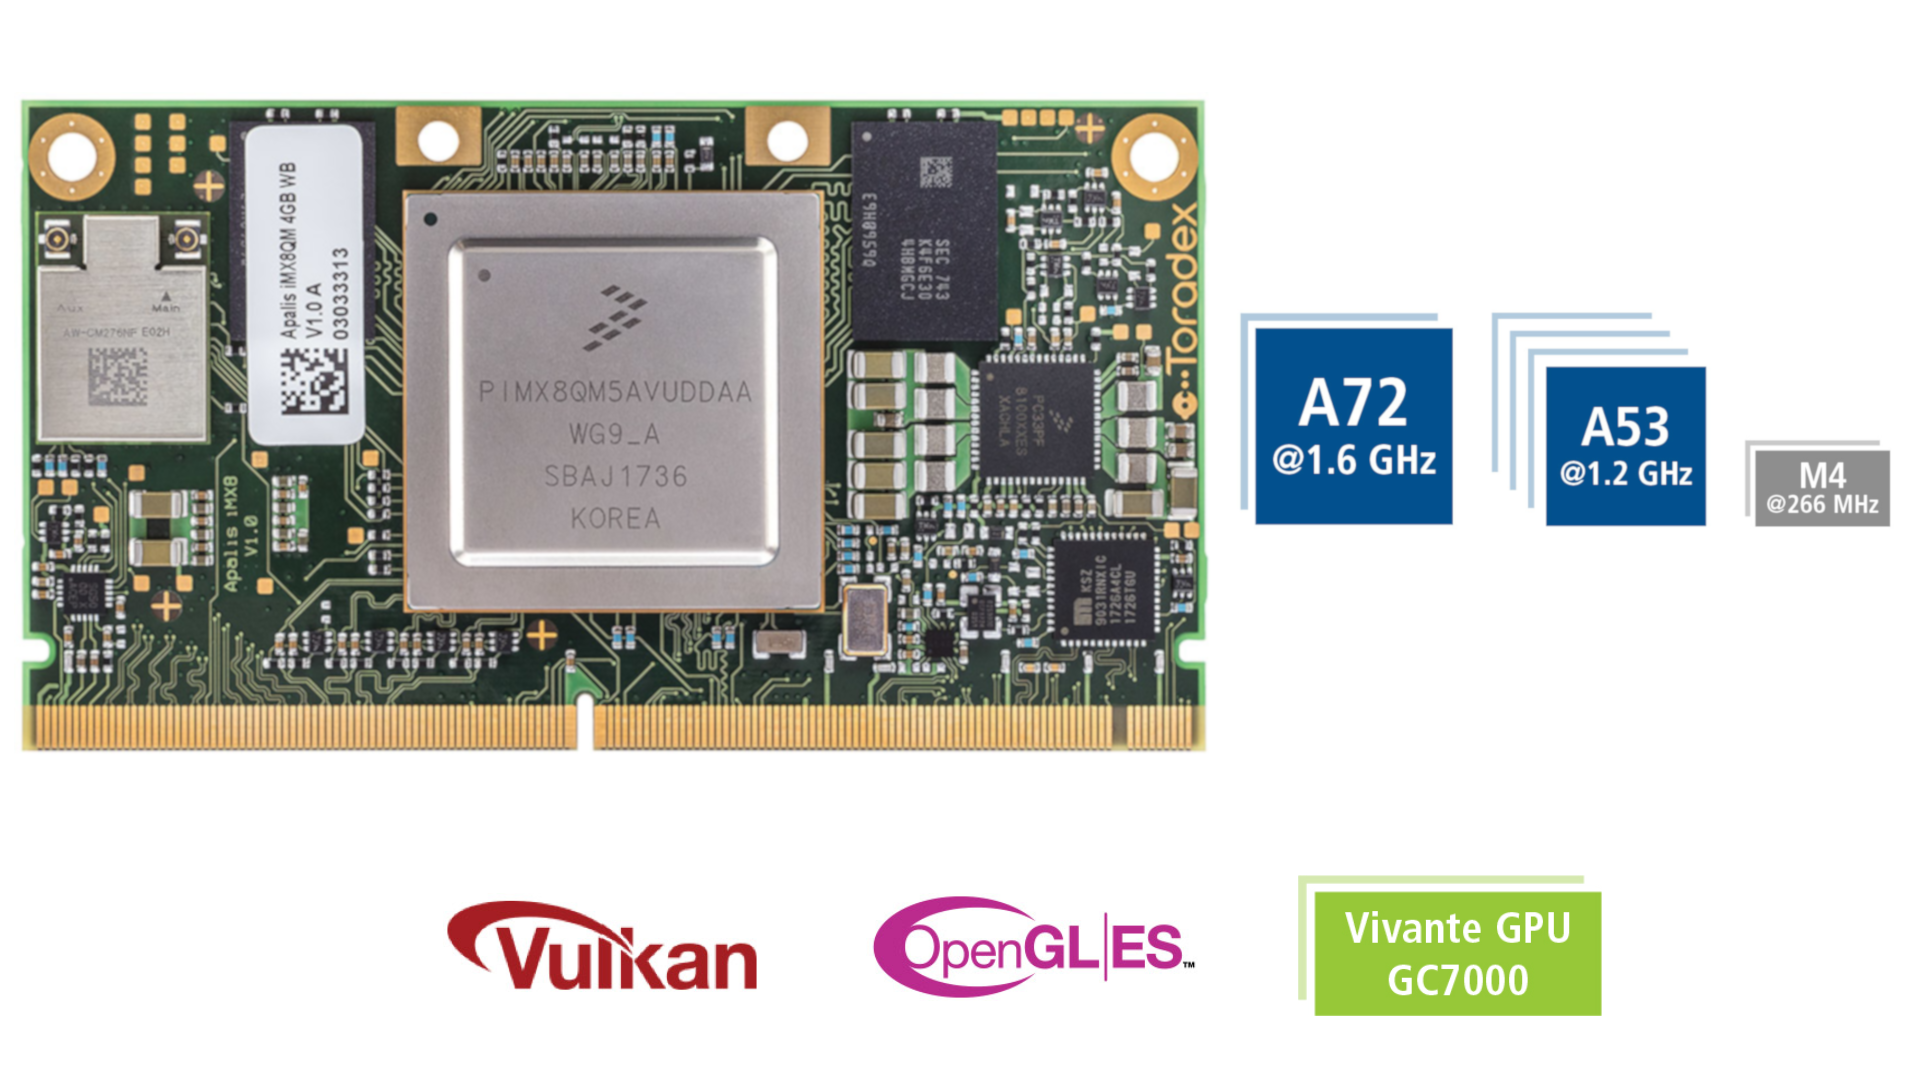
\includegraphics[height=0.9\textheight]{./img/apalis_imx8_slide.png}
  \end{center}
\end{frame}

\note{
}

\begin{frame}{Why Apalis iMX8?}
  \begin{center}
    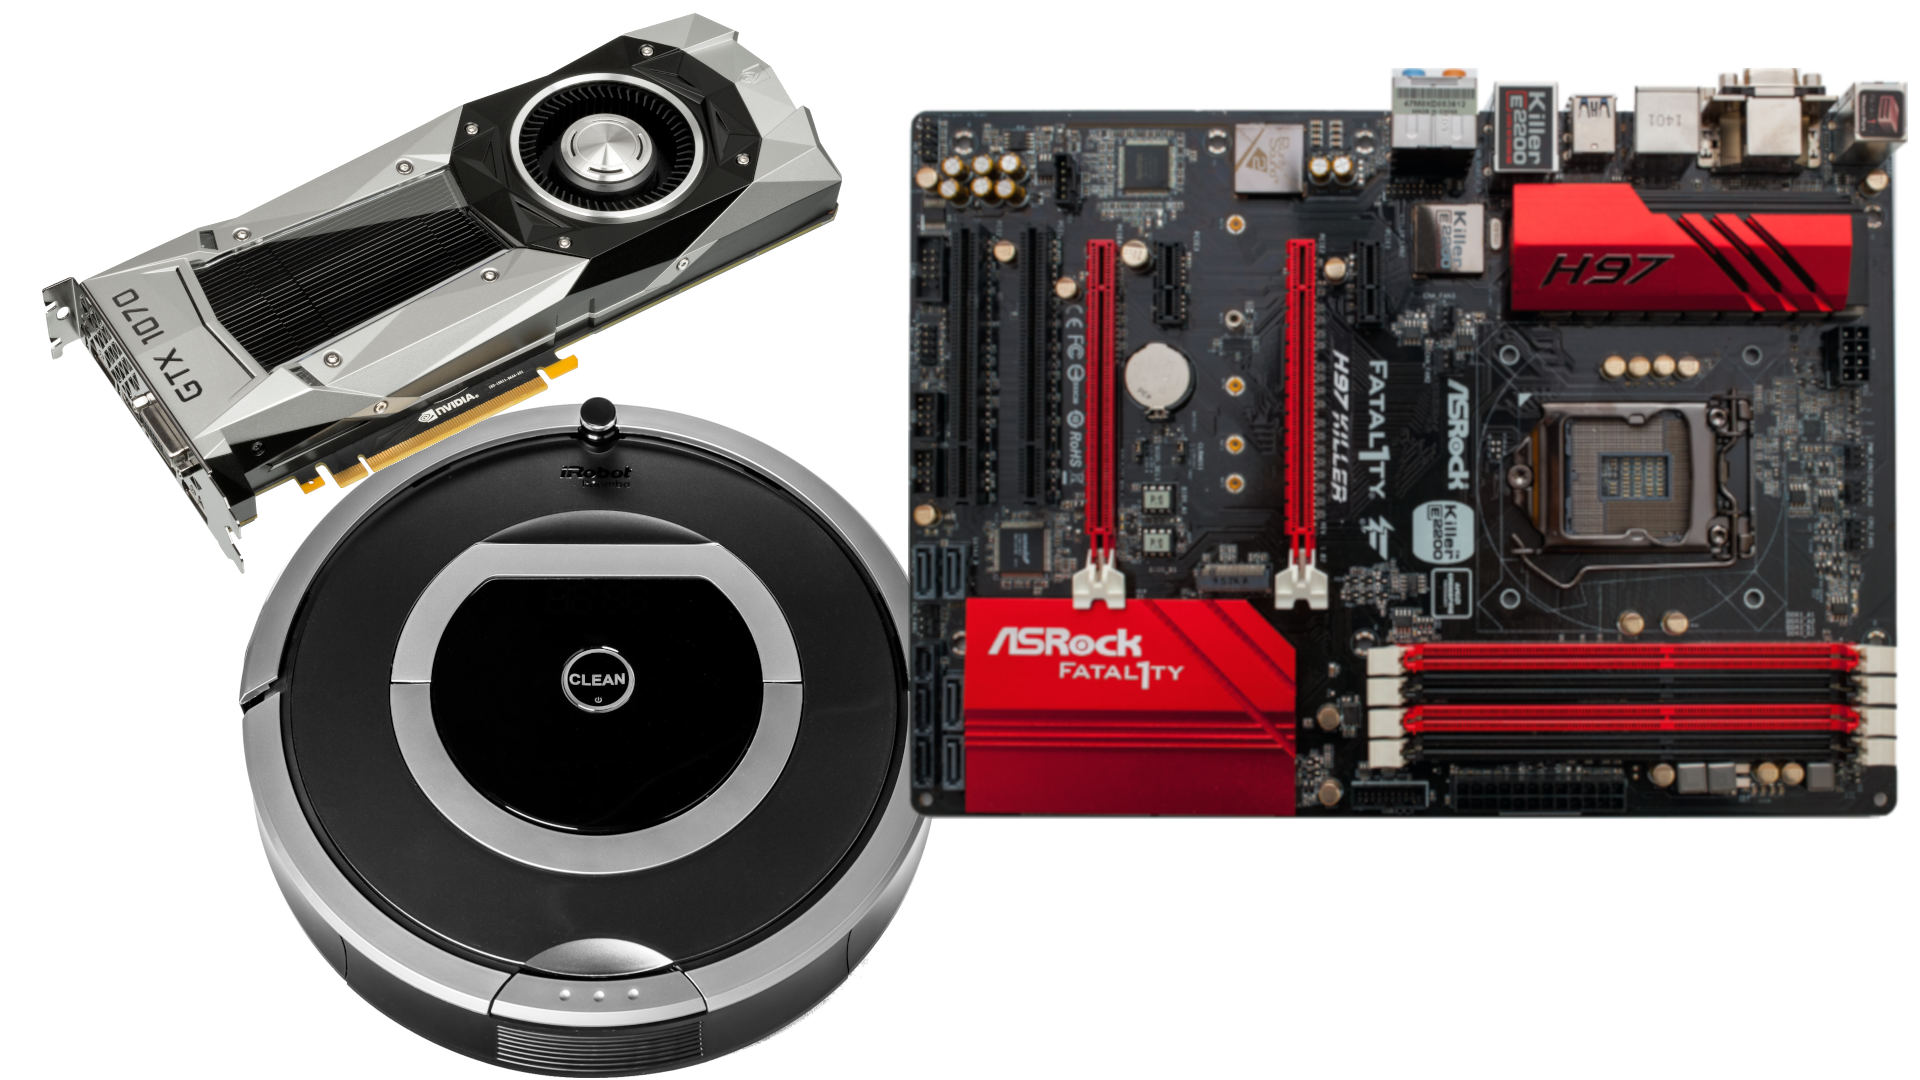
\includegraphics[height=0.9\textheight]{./img/robot_size.png}
  \end{center}
\end{frame}

\note{
}

\begin{frame}{Different SLAMs}
  \begin{center}
    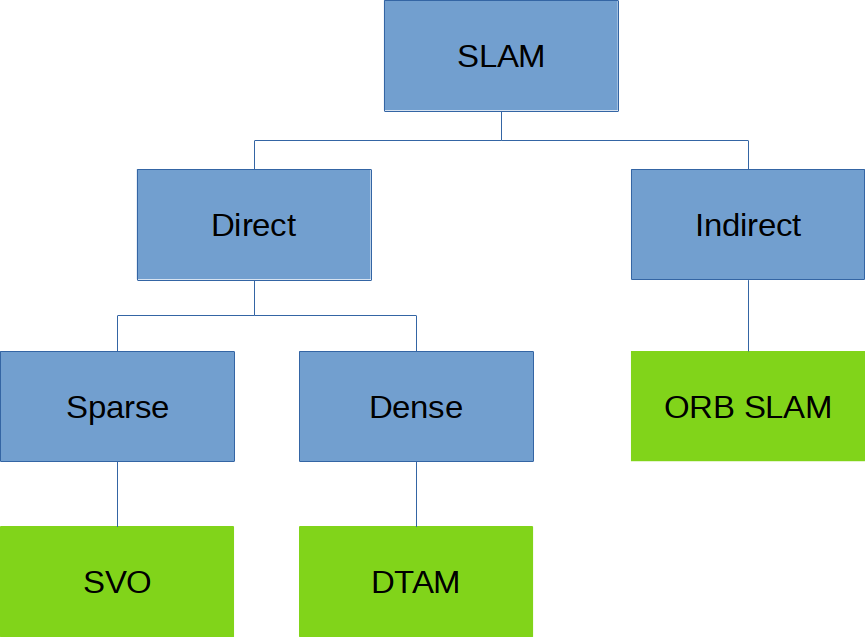
\includegraphics[height=0.9\textheight]{./img/slam_modes.png}
  \end{center}
\end{frame}

\note{
}

\begin{frame}{Stereo Camera}
  \begin{center}
    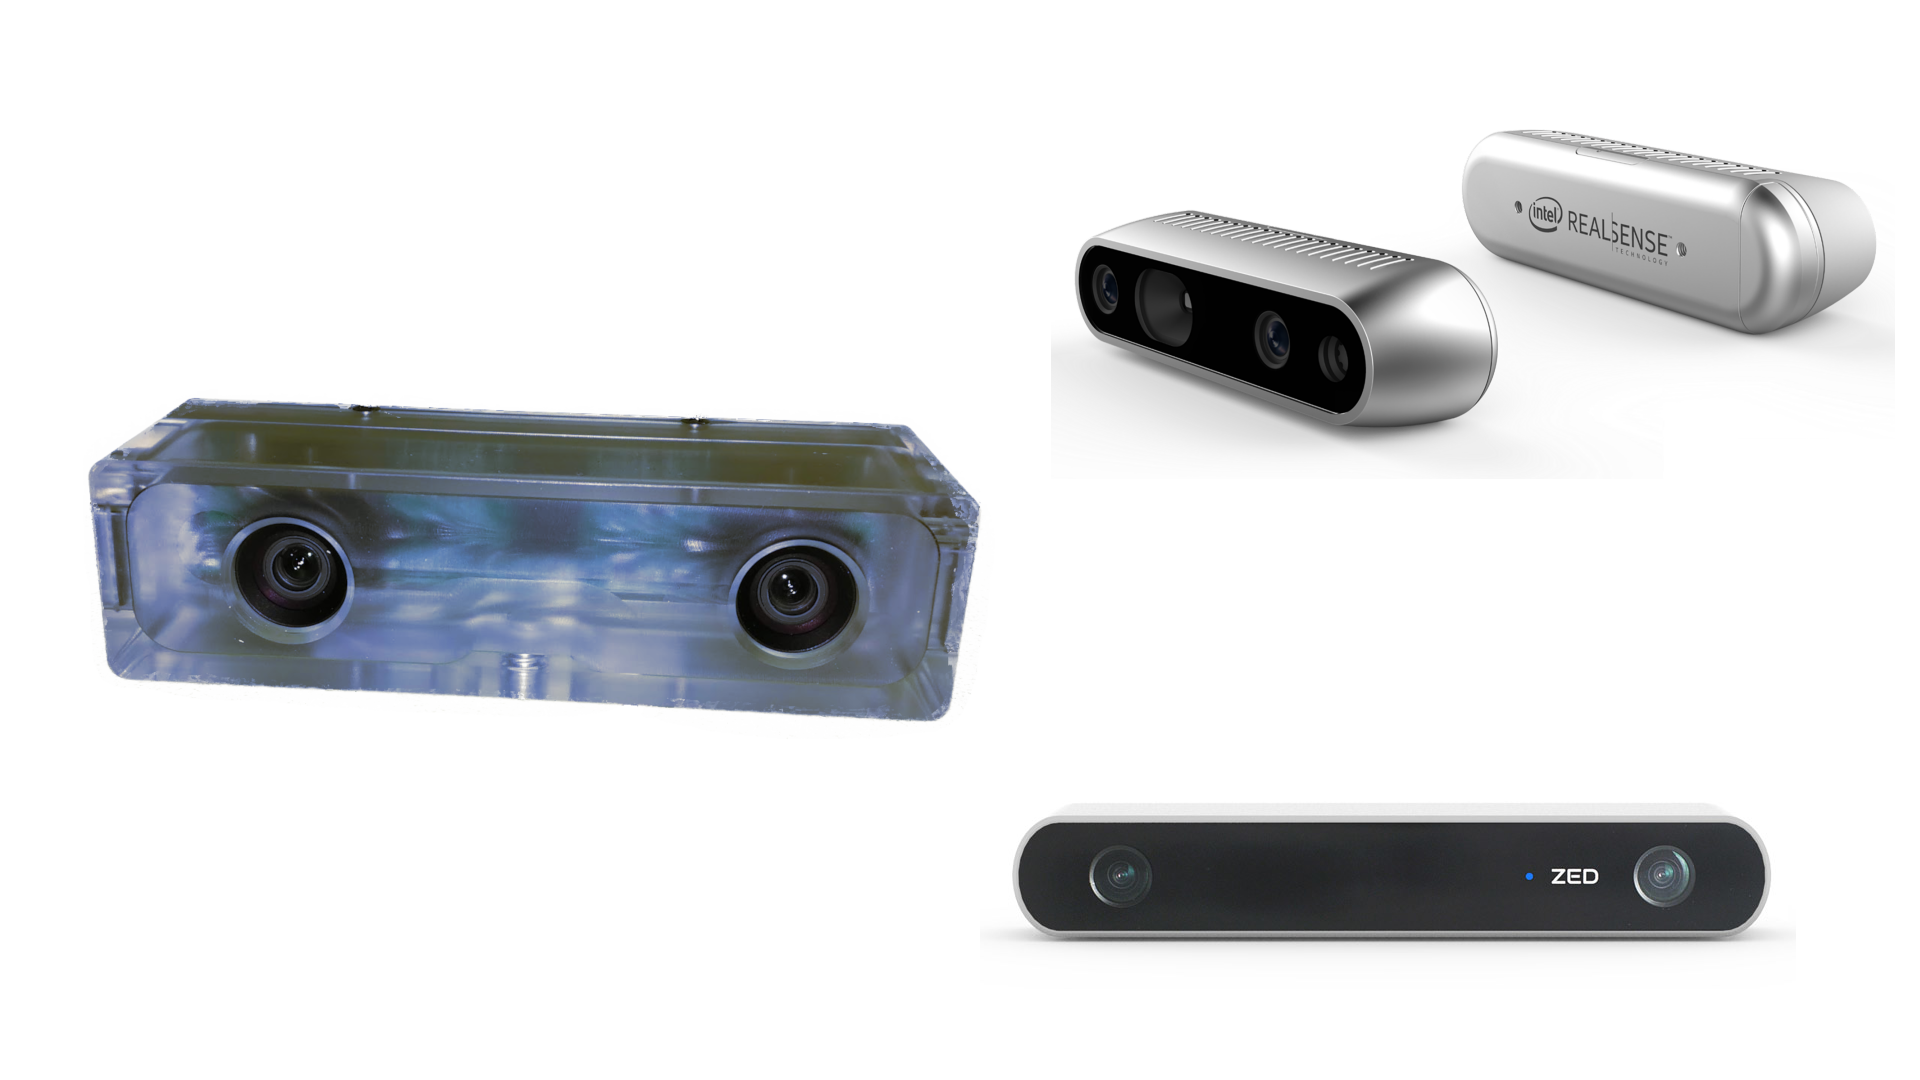
\includegraphics[height=0.9\textheight]{./img/cameras.png}
  \end{center}
\end{frame}

\note{
}


\begin{frame}{Stereo Calibration}
  \begin{center}
    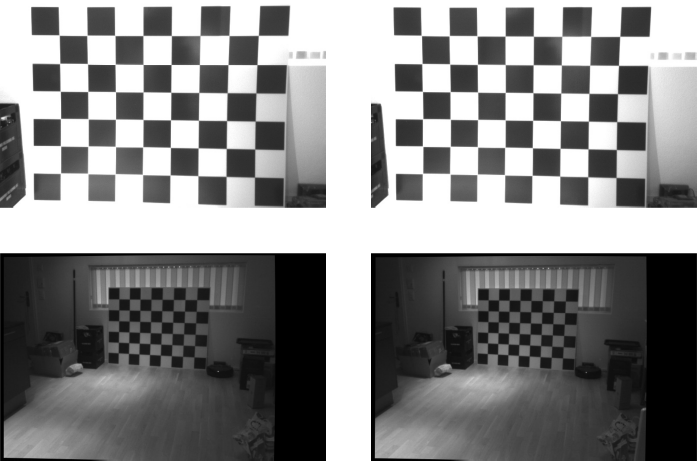
\includegraphics[height=0.9\textheight]{./img/stereo_calib.png}
  \end{center}
\end{frame}

\note{
}

\begin{frame}{Depth from Stereo}
  \begin{center}
    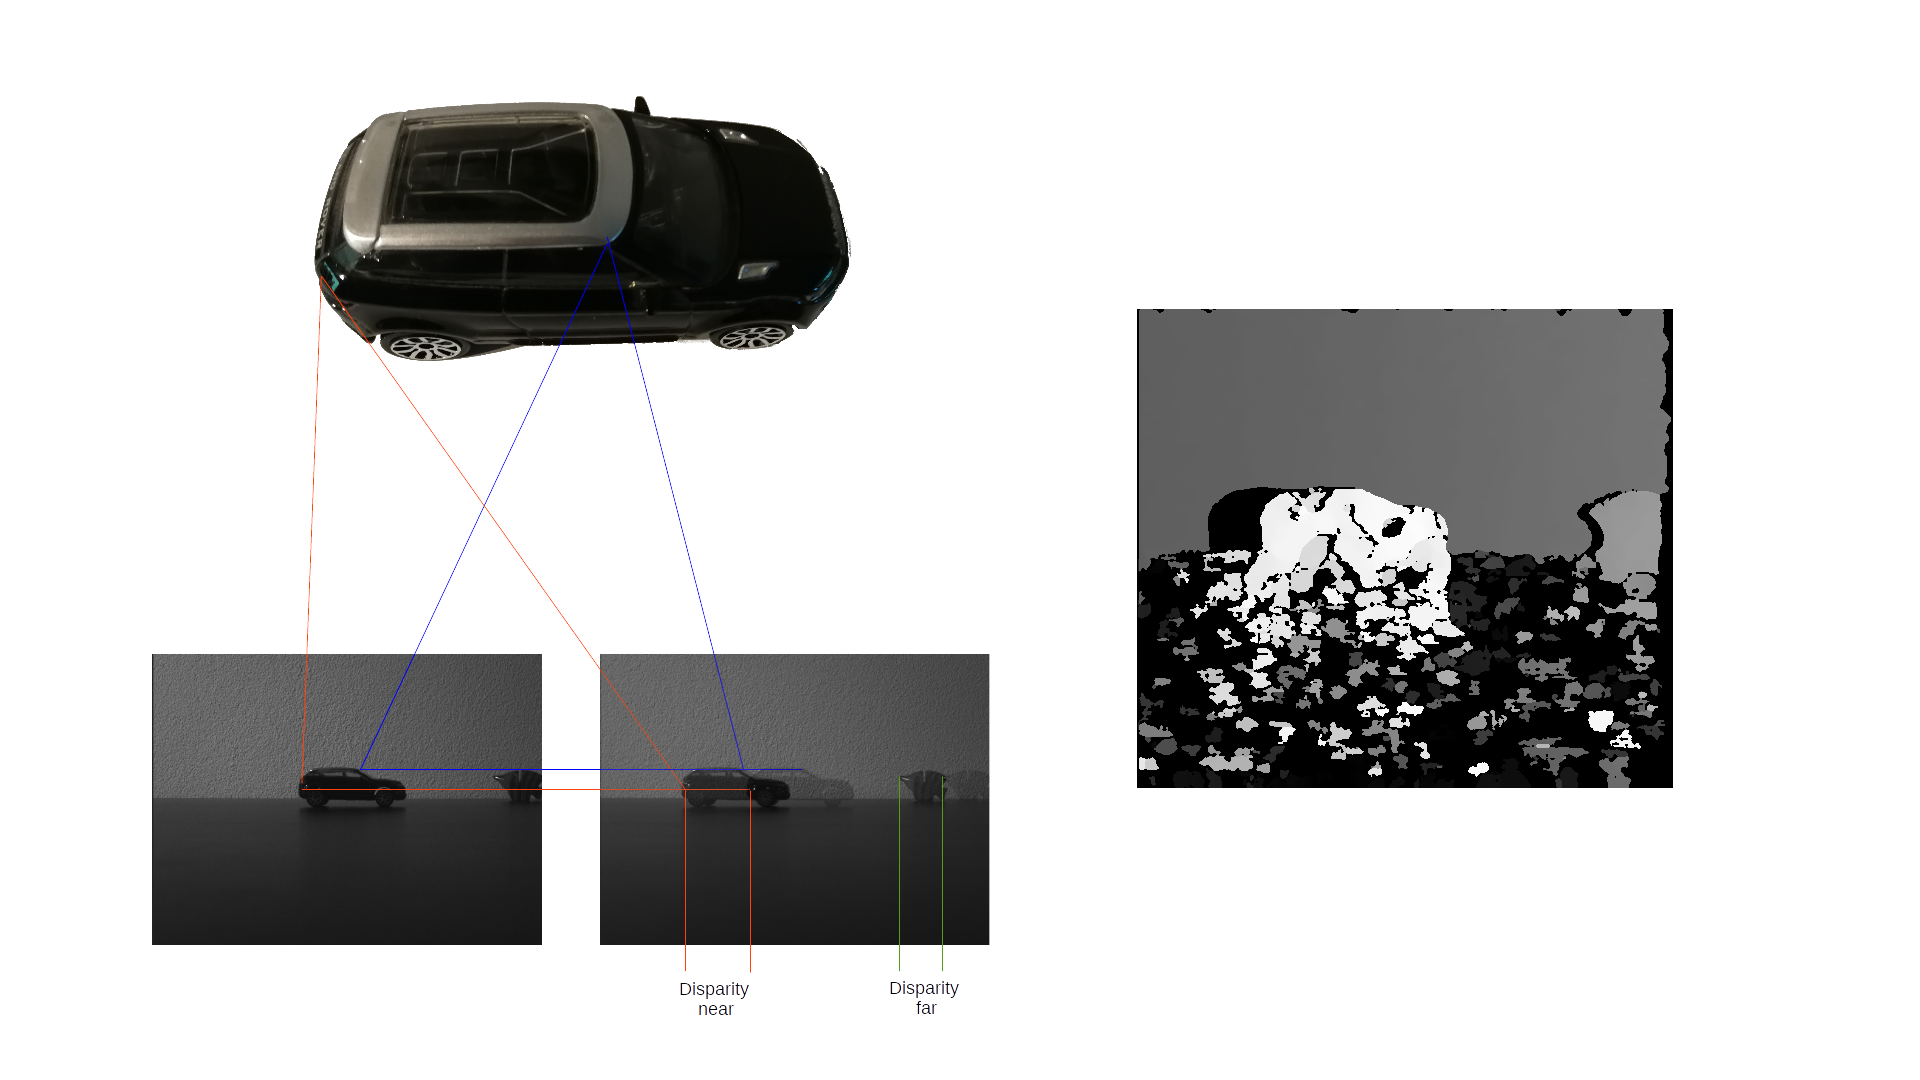
\includegraphics[height=0.9\textheight]{./img/disparity.png}
  \end{center}
\end{frame}

\note{
}


\begin{frame}{ORB SLAM}
  \begin{center}
    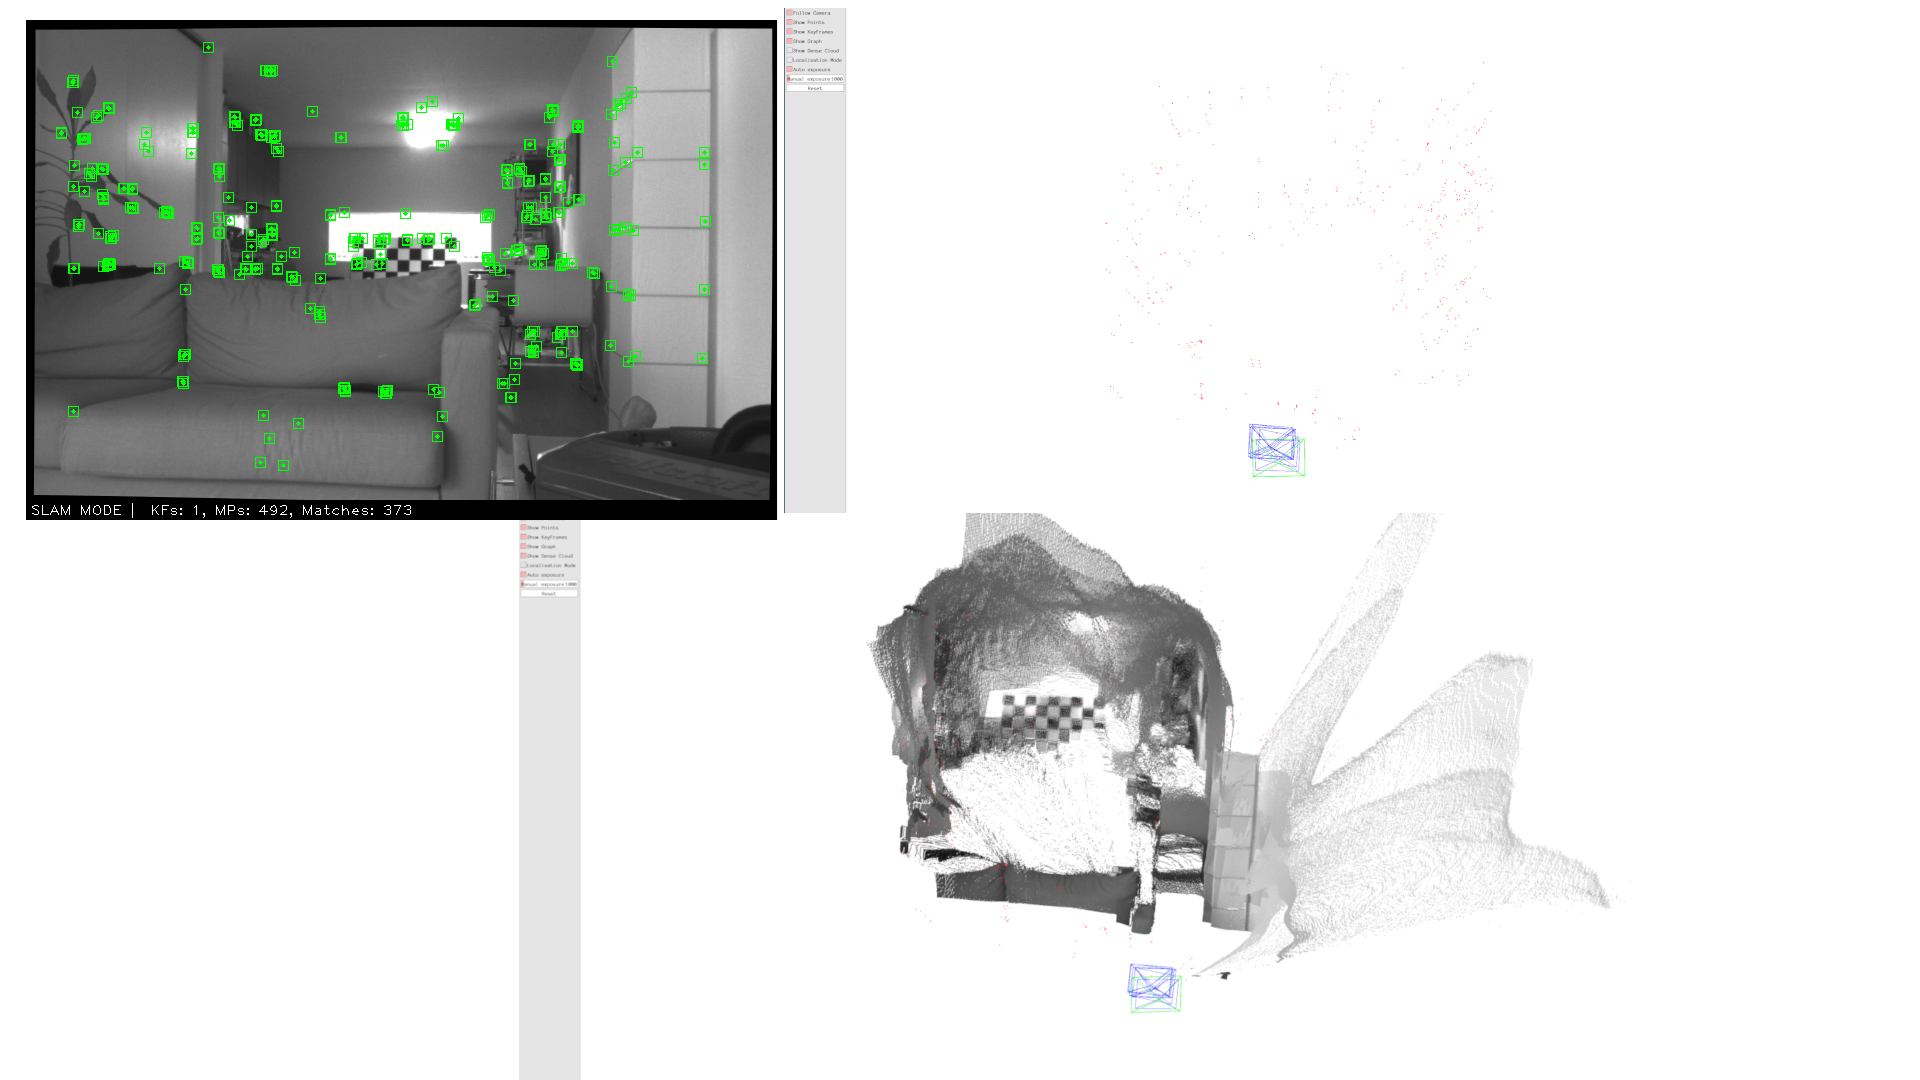
\includegraphics[height=0.9\textheight]{./img/orbslam.png}
  \end{center}
\end{frame}

\note{
}

\begin{frame}{Densification}
  \begin{center}
    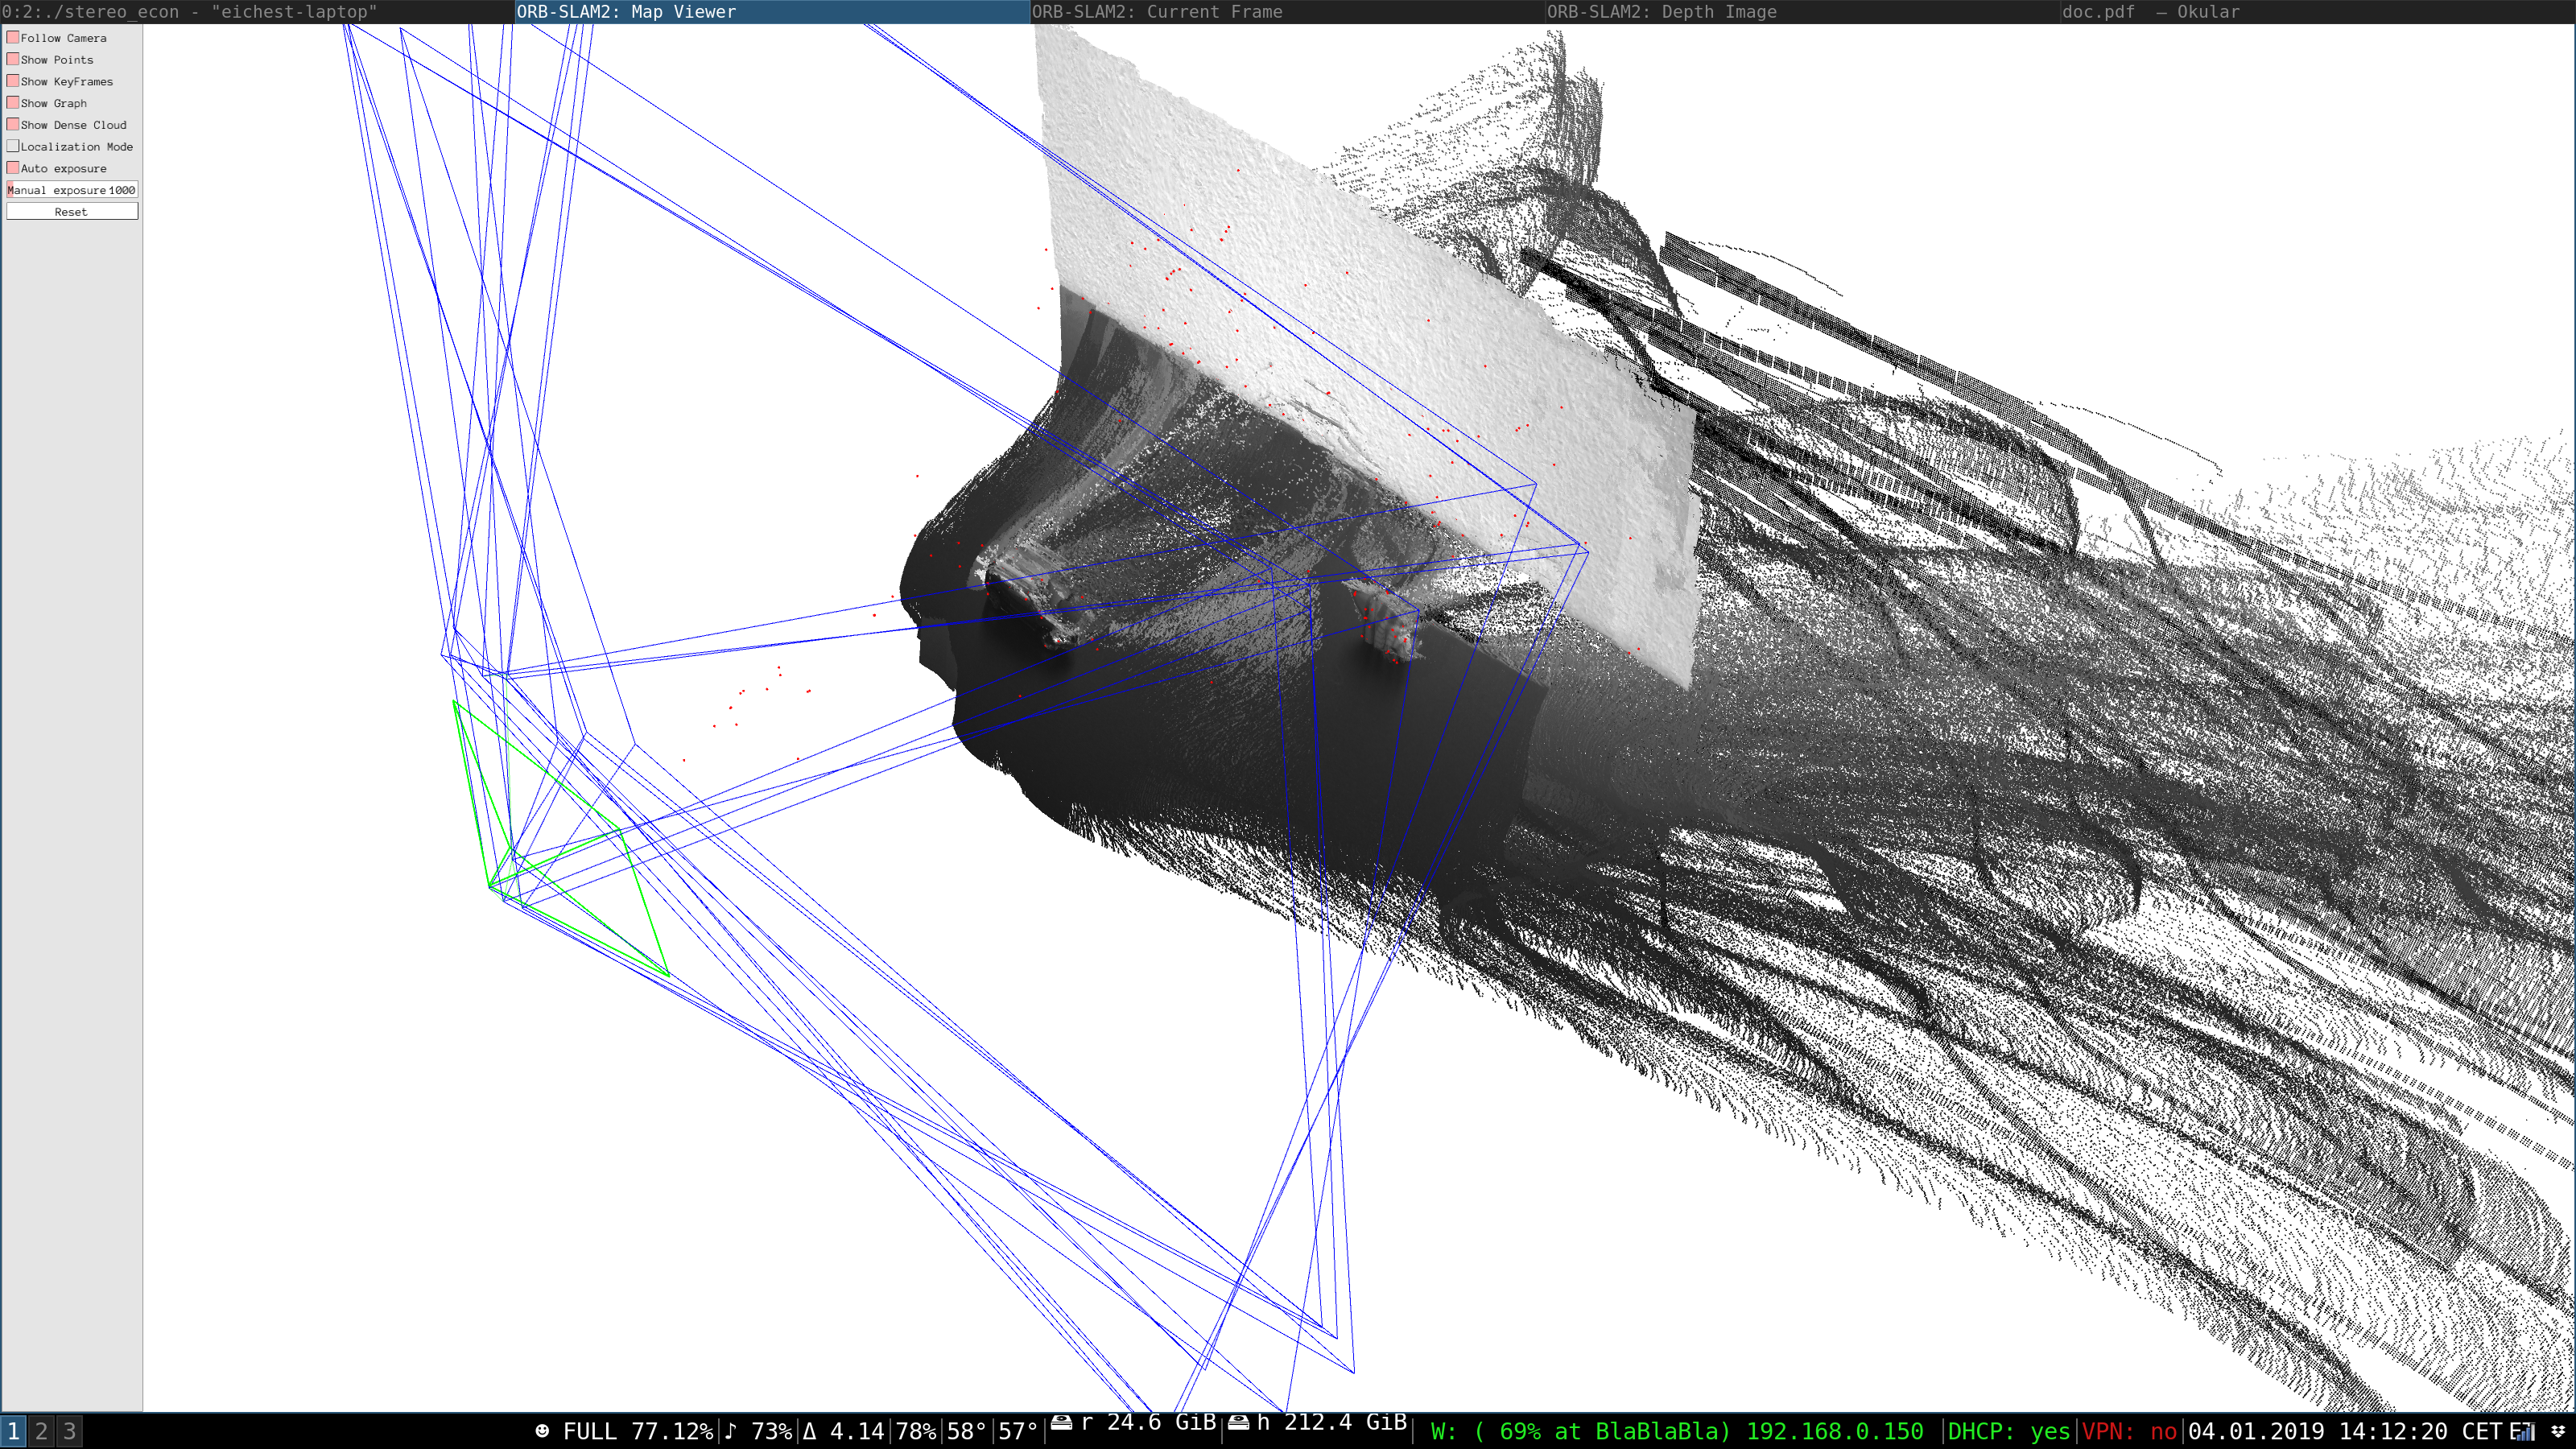
\includegraphics[height=0.9\textheight]{./img/pointcloud.png}
  \end{center}
\end{frame}

\note{
}

\begin{frame}{Results (KITTI 04 Dataset)}
  \begin{center}
  \begin{table}
    \begin{tabular}{ l | l | l | l | l | l  }
      \textbf{CPU} & \textbf{Impl.} & \textbf{feat.} & \textbf{feat. det.} & \textbf{med. tt} & \textbf{mean tt} \\ \hline
      iMX8 & ORB & 1000 &  548 & 0.18307 & 0.185202 \\ \hline
      iMX8 & ORB, Lin. sched. & 1000 & 548 & 0.390867 & 0.387753 \\ \hline
      iMX8 & OpenCV & 1000 & 757 & 0.190571 & 0.210072 \\ \hline
      iMX8 & OpenCV & 800 & 610 & \textbf{0.155441} & \textbf{0.167176} \\ \hline
      iMX8 & OpenCV, Lin. sched. & 800 & 610 & 0.358689 & 0.362126 \\ \hline
      iMX8 & OpenCV OpenCL & 800 & 610 & 0.50622 & 0.771859 \\ \hline
      i5-7Y54 & ORB & 1000 & 546 & 0.18884 & 0.184628 \\ \hline
      i5-7Y54 & OpenCV & 1000 & 756 & 0.154901 & 0.152786 \\ \hline
      i5-7Y54 & OpenCV & 800 & 610 & 0.135715 & 0.132304 
    \end{tabular}
  \end{table}
\end{center}
\end{frame}

\note{
}

\begin{frame}{Demo}
  \begin{center}
  \end{center}
\end{frame}

\note{
}

\begin{frame}{Direct Approach}
  \begin{center}
    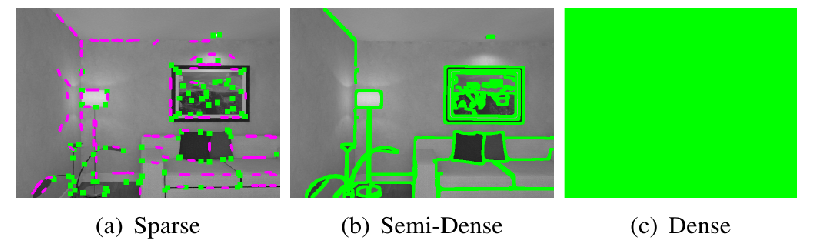
\includegraphics[width=0.9\textwidth]{./img/sparse_dense.png}
  \end{center}
\end{frame}

\note{
}

\begin{frame}{Questions}
  \begin{center}
    
\includegraphics[height=0.9\textheight]{./img/question.jpg}
  \end{center}
\end{frame}


\end{document}

